% Define document class

\PassOptionsToPackage{table}{xcolor}

\documentclass[twocolumn]{aastex631}
\usepackage{showyourwork}
\usepackage{amsmath}
\usepackage{xcolor}
\usepackage{booktabs}
\usepackage{todonotes}

\newcommand{\mrm}[1]{\mathrm{#1}}
\newcommand{\mbs}[1]{\boldsymbol{#1}}
\newcommand{\mbf}[1]{\mathbf{#1}}
\newcommand{\mbb}[1]{\mathbb{#1}}
\newcommand{\mfk}[1]{\mathfrak{#1}}
\newcommand{\mcal}[1]{\mathcal{#1}}
\newcommand{\unit}[1]{[\text{#1}]}

\newcommand{\nth}[1]{{#1}_{\mrm{n}}}
\newcommand{\fth}[1]{{#1}_{\mrm{f}}}
\newcommand{\qth}[1]{{#1}_{\mrm{q}}}

\newcommand{\pdf}{P}
\newcommand{\cdf}{\Phi}

\newcommand{\Exp}[1]{e^{#1}}
\newcommand{\Erf}[1]{\mathrm{erf}\left(#1\right)}

\newcommand{\sigobs}{{\sigma_*}}
\newcommand{\JN}[1]{{\textcolor{red}{JN: #1}}}

\NewDocumentCommand \dif {o m} {
	\IfNoValueTF{#1}
		{ \mathrm{d}{#2} }
		{ \mathrm{d}^{#1}{\!#2} }
}

% Begin!
\begin{document}

% Title
\title{Characterizing Stellar Streams by ML}

% Author list
\author{Nathaniel Starkman}
\author{Jacob Nibauer}
\author{Jo Bovy}
\author{Jeremy Webb}

% Abstract with filler text
\begin{abstract}
    Stellar stream membership likelihoods with ML. It works!
\end{abstract}

\section{Introduction} \label{sec:intro}

    [Content Here]

    \

    Paper Map:
    \begin{enumerate}
        \item Intro
        \item Method \begin{enumerate}
            \item Fig 1: Overall explainer figure that illustrates the method with Neural networks, and norm flow for CMD
            \item Fig 2: Bayesian graphical model
            \item Test On Synthetic Stream:
            \item Some sort of plot demonstrating successful recovery
        \end{enumerate}
        \item Application / Results \begin{enumerate}
            \item Test case GD-1: \begin{enumerate}
                \item CMD norm flow background
                \item Fig: Stream phi1 phi2 top panel and histograms of each dimension below GD-1
                \item Some plot in phi1-phi2 that shows density variations
            \end{enumerate}
            \item Test case Pal-5 \begin{enumerate}
                \item CMD norm flow background
                \item Fig: Stream phi1 phi2 top panel and histograms of each dimension below Pal 5
                \item Some plot in phi1-phi2 that shows density variations
            \end{enumerate}
        \end{enumerate}
        \item Conclusion
        \item Appendix
    \end{enumerate}

% section introduction (end)

\section{Method} \label{sec:method}


    Stellar streams 

    \subsection{Likelihood Setup}\label{sub:likelihood_setup}
    
        \begin{figure}
        \centering
        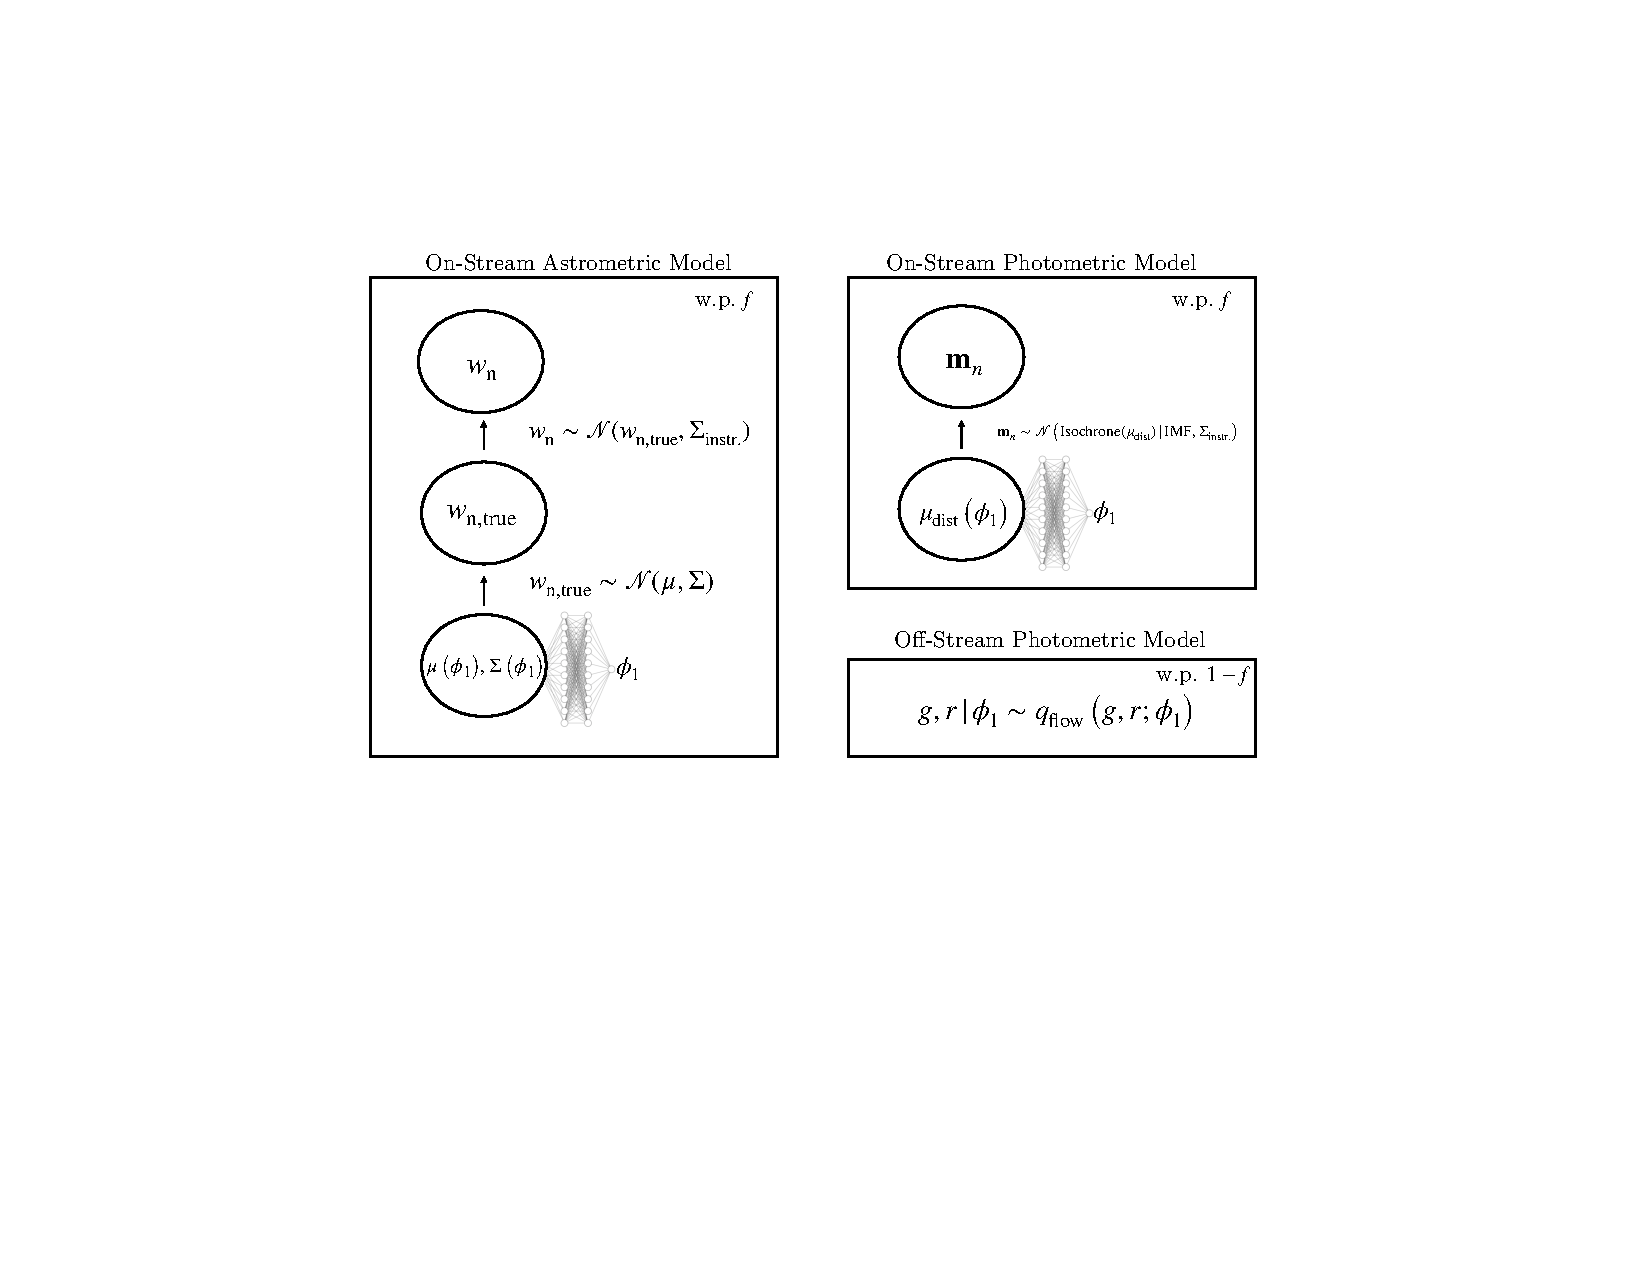
\includegraphics[scale=0.5]{figures-not-syw/DAG_StreamDensity.pdf}
        \caption{Fill in.}
        \label{fig: DAG}
        \end{figure} 
    
        We model the stream and background as functions continuous in some affine parameter. In principle this parameter can be anything. Though it might seem the best parameter is the stream's arc length, the most common, easiest, and practical parameter is the longitude -- $w_{\cdot, j\equiv0} \equiv \phi_1$ -- in some stream-oriented reference frame \citep[for details see][section 2]{2023MNRAS.522.5022S}.


        

        We model the likelihood for a single star as
        \begin{align} \label{eq:general_model}
            \pdf(\nth{\mbs{w}}, \nth{\mbs{m}} | \mbs{\theta})
                &= \sum_{q} \ f_q(w_{i, 0}) \pdf(\nth{\mbs{w}}|\mbs{\theta},q_i\!=\!q) \pdf(\nth{\mbs{m}}|\mbs{\theta},q_i\!=\!q)
        \end{align}
        where we have assumed that $\nth{\mbs{w}}$ and $\nth{\mbs{m}}$ are conditionally independent, and that the mixture weights $f$ are normalized s.t. $\sum_q f(w_{i,0}) = 1$. We discuss the mixture weights further in \autoref{sub:mixture_weight}

        Assuming the measurement of each star is independent, the total log-likelihood is a sum over all stars:
        \begin{equation}
            \ln\mcal{L}\left(\{(\nth{\mbs{w}},\nth{\mbs{m}})\} | \mbs{\theta}\right) = \sum_i  \ln \pdf(\nth{\mbs{w}}, \nth{\mbs{m}} | \mbs{\theta}).
        \end{equation}

        It will prove convenient to distinguish the models for $q=0,1$ as the \textit{background} and \textit{stream} models, respectively. In this notation:

        \begin{multline}
            \pdf(\nth{\mbs{w}}, \nth{\mbs{m}} | \mbs{\theta}) 
            = \\\phantom{+} \ \quad f \quad\ P^{(S)}(\nth{\mbs{w}}|\mbs{\theta}) P^{(S)}(\nth{\mbs{m}}|\mbs{\theta})  \\
            \quad + (1-f) P^{(B)}(\nth{\mbs{w}}|\mbs{\theta}) P^{(B)}(\nth{\mbs{m}}|\mbs{\theta}), \nonumber
        \end{multline}

        The probablity of a being a stream member is then simply
        \begin{equation}\label{eq:membership_prob}
            \pdf\left(S | \mbs{w}_n, \mbs{m}_n, \mbs{\theta} \right) = \frac{f P^{(S)}(\nth{\mbs{w}}|\mbs{\theta}) P^{(S)}(\nth{\mbs{m}}|\mbs{\theta}) }{ \pdf(\nth{\mbs{w}}, \nth{\mbs{m}} | \mbs{\theta})}.
        \end{equation}
    Hereafter, when we refer to ``membership probability," Eq.~\ref{eq:membership_prob} provides the formal definition. 
    %\newpage

    \subsection{Determination of the Mixture Weight} \label{sub:mixture_weight}
        The mixture weight $f_q(w_{i,0})$ as used in Eq.~\ref{eq:general_model} is characterized as the fraction of stars belonging to the mixture component $q$ over an increment $[w_{i,0}, w_{i,0} + \dif{w_{i,0}}]$. Thus, the mixture weight encodes information about the linear density of the stream, which has been shown to depend on substructure in the galaxy (CITE-x). The dependence of the mixture weight on the linear density is captured by the expression
        \begin{equation}\label{eq:fraction_param}
            f_q\left(w_{i,0}\right) = \frac{N_q\left(\phi_1\right)}{N_{\rm tot}\left(\phi_1\right)},
        \end{equation}
        where $N_q\left(\phi_1\right)$ is the number of stars in component $q$ within an interval $[\phi_1, \phi_1 + \dif{\phi_1}]$, and 
        $N_{\rm tot}$ is the total number of stars in the same band (including those in component $q$). The linear  density for component $q$ is then entirely specified by the function $N_q(\phi_1)$.

        The mixture model specified in \S-X only models the weight parameter $f_q$, and not the components of the ratio in \autoref{eq:fraction_param}. However, the linear density $N_q(\phi_1)$ can be readily obtained from $f_q$, provided that $N_{\rm tot}\left(\phi_1\right)$ can be calculated. Importantly, this function does not depend on the parameters of the on-stream or off-stream model. Instead, $N_{\rm tot}(\phi_1)$ is simply the number of stars in a small $\phi_1$ increment. We therefore model $N_{\rm tot}\left(\phi_1\right)$ as a post-processing step using a single normalzing flow in $\phi_1$. 

        In particular, for a given field the distribution of $\phi_1$ coordinates is specified by the set $\{\phi_{1,i}\}_i$. A normalizng flow is trained to this dataset, and will satisfy $\int d\phi_1 P_{\phi_i}(\phi_1) = 1$ by construction. In order to re-weight the normalizing flow to obtain $N_{\rm tot}(\phi_1)$, we simply rescale $P_{\phi}(\phi_1)$ by $N_{\rm tot,0}$, which is the total number of stars in the field considered. We can then obtain the linear stream density with
        \begin{equation}
            N_q\left(\phi_1\right) = f_q N_{\rm tot} \left(\phi_1\right)  = f_q \left[N_{\rm tot,0} P_{\phi_1}\left(\phi_1\right) \right] .
        \end{equation}

    
        
    \subsection{Astrometric Model} \label{sub:astrometric_model}

        \subsubsection{On-Stream} \label{ssub:astrometric_model_on_stream}
    
            The astrometric track is modeled with a neural network, encompassing each phase space dimension, parameterized as a function of $\phi_1$. The neural network output for a single stream component is the mean location of the stream track in each dimension, $\mbs{\mu}_w(\phi_1 | q_i)$, and its associated covariance matrix $\mbs{\Sigma}_w(\phi_1 | q_i)$. The probability for the data is then
            \begin{equation}
                \pdf^{(S)}(\nth{\mbs{w}} | \mbs{\theta}, \phi_{1,i}, q_i) = \mcal{N}\big(\nth{\mbs{w}} | \mbs{\mu}_w\left(\phi_{1,i} | q_i \right), \mbs{\Sigma}_w\left(\phi_{1,i} | q_i \right) \big),
            \end{equation}
            where $\mbs{\theta}$ is the set of neural network parameters that define $\mbs{\mu}_w$ and $\mbs{\Sigma}_w$.
            In the simplest case, we take $\mbs{\Sigma}_w$ to be diagonal, consisting of both intrinsic dispersion for each dimension of $\mbs{w}$ and the data uncertainties added in quadrature. 

            In practice, we work with truncated Gaussians, where the truncation is set by the size of the field in each astrometric dimension. This ensures that the probability density is zero wherever there is no data. Details of the truncated Gaussian are included in \autoref{app:distributions}.

        \subsubsection{Off-stream} \label{ssub:astrometric_model_off_stream}
    
            We now outline the off-stream astrometric model. We take a similar approach to the on-stream astrometric model discussed in \S\ref{ssub:astrometric_model_on_stream}, though we typically do not characterize the backgrounds with a Gaussian distribution. Instead, we utilize a range of distributions (i.e., exponential, skew-normal) discussed in \autoref{app:distributions}. The parameters of the user-specified background distributions are themselves neural network outputs, such that any $\phi_1$ ``slice" of the background should be characterized by some analytic density, but the evolution of the backgrounds with $\phi_1$ can be complex. 
    
            Let $\mbs{\theta}_{B,j}(\phi_1)$ represent the neural network which outputs a vector of parameters characterizing the background distribution at a given $\phi_1$ for astrometric dimension $j$. The number of outputs for the background model is equal to $\Sigma_{j>0} \mathrm{dim}\left(\mbs{\theta}_{B,j}\right)$ (where $j=0$ corresponds to $\phi_1$, which we do not model). At a given $\phi_1$, the probability density for the astrometric dimension $j>0$ is $\pdf^{(B)}_j\left(\mbs{w}_{n,j} | \mbs{\theta}, \mbs{\theta}_{B,j}, \phi_1 \right)$. We treat each background component as independent, allowing us to write the likelihood as a product over the astrometric dimensions:
            \begin{equation}
                \pdf^{(B)}\left(\mbs{w}_n | \mbs{\theta}, \phi_1 \right) = \prod_{j>0} \pdf_j^{(B)}\left(\mbs{w}_{n,j} | \mbs{\theta}, \mbs{\theta}_{B,j}, \phi_1 \right).
            \end{equation}
    

        

    
    
        
        
    %\newpage

    \subsection{Photometric Model} \label{sub:photometric_model}

        \subsubsection{On-Stream} \label{sub:photometric_model_on_stream}
            In photometric coordinates we model the stream as a single-population isochrone with the possibility of a non-zero distance gradient. We accomplish this by modeling the distance of the isochrone as a neural network output, parametrized as a function of $\phi_1$. The result is a distance track along the stream, estimated from the variation in its isochrone with $\phi_1$. 
            
            At any given $\phi_1$, the isochrone is modeled in absolute magnitudes
            and parameterized by the unit-normalized stellar mass, labeled $\gamma$. For example, increasing $\gamma$ corresponds to movement up the main sequence towards the red giant branch. We denote the isochrone as $\mcal{I(\gamma)}$. The intrinsic dipsersion around the isochrone is $\Sigma_\mcal{I}(\gamma)$. Since the isochrone is in absolute magnitudes, but the data are in apparent magnitudes,
            it is necessary to shift the isochrone by a distance modulus to the predicted distance of the stream, labeled  $\mu(\nth{\phi_1})$.
            
            For the $n$-th star, the photometric model is:
    
            \begin{multline}
                P^{(S)}(\mbs{m_i}, \gamma; \mbs{\theta}(\nth{\phi_1}), \nth{\phi_1}) 
                \\ \sim \mcal{N}(\nth{\mbs{m}}; \{\mcal{I(\gamma)} + \mu(\nth{\phi_1}), \sqrt{\Sigma_{\mcal{I}}^2(\gamma) + \Sigma_\mu^2(\nth{\phi_1}) + \Sigma_i^2} \}) \\ \times\pdf(\gamma, \nth{\phi_1}),
            \end{multline}
    
            where $\pdf(\gamma)$ encodes both the present-day mass function of the stream, as well as the observational constraints (e.g. $g < 22$ mag).
    
            We are interested in the total probability (at some $\phi_1$) and so integrate over $\gamma$ to find:
            \begin{small}
            \begin{multline}
                P^{(S)}(\nth{\mbs{m}}; \mbs{\theta}(\nth{\phi_1}), \nth{\phi_1}) = \\\int\limits_{\gamma=0}^{1} \mcal{N}(\mbs{m}; \{\mcal{I(\gamma)} + \mu(\nth{\phi_1}), \sqrt{\Sigma_{\mcal{I}}^2(\gamma) + \Sigma_\mu^2(\nth{\phi_1}) + \Sigma_i^2} \}) \pdf(\gamma) \rm{d}\gamma.
            \end{multline}\end{small}
            Then, for a given $\phi_1$ we can obtain a distribution over the distance modulus using 
            \begin{equation}
                \mu_{\rm sample}\left(\phi_1\right) \sim \mathcal{N}\left(\mu(\phi_1), \Sigma^2_\mu(\phi_1) \right) \quad\unit{mag}.
            \end{equation}
            For each sample, we can convert the distance-modulus distribution to the distance track using 
            \begin{equation}
                \rm{dist}\left(\phi_1\right) = 10^{\frac{1}{5}\mu_{\rm sample}(\phi_1)+1} \quad\unit{pc}.
            \end{equation}

            \todo[inline]{TODO:}
            \begin{enumerate}
                \item Not including isochrone parameters, e.g. age and metallicity
                \item integrating over $\gamma$ the model assumes a PDMF, e.g. Kroupa
            \end{enumerate}

            By integrating over $\gamma$ the model is not sensitive to 

    
        \subsubsection{Off-stream} \label{sub:photometric_model_off_stream}
            In this section we introduce our model for the distribution of backgrounds in photometric coordinates. 

            In general, the distribution of stars in color (i.e., $g-r$) and magnitude (i.e., $g$) is a complicated function of location in the galaxy. Even within a field centered on the stream of interest, the color-magnitude diagram (CMD) is a combination of stellar populations distributed over a range in distances. Because of this, we do not expect an analytic density to provide a realistic description of the data. In this work we take a data-driven approach, and represent the CMD using a normalizing flow model.

            Normalizing flows provide a flexible description of a probability density, by transforming samples generated from a simple base distribution (i.e., a Gaussian) to the more complicated target distribution. The transformations are typically non-linear outputs of a neural neural network, whose parameters are optimized until the target density accurately characterizes the data. The neural network transformation is differentiable, so that jacobian factors can be combined to ensure that the the target distribution remains a valid probability density (i.e., integrates to one).  

            Our implementation is as follows. For a given stream, we restrict the data to some field characterized by a polygon drawn around the stream. Because our density modeling is aimed at stream characterization rather than discovery, we assume that the stream is sufficiently well known so that it can be masked out as a simple cut in (e.g.) $\phi1-\phi_2$ coordinates. With the stream masked out, we then fit a normalizing flow to the photometric data. Because the background CMD can evolve with $\phi_1$, we fit a \emph{conditional} normalizing flow, $q_{\rm flow}(\mathbf{m}|\phi_1)$, so that the color-magnitude diagram is conditionally dependent on position along the stream. In practice, we model magntiudes and not colors (i.e., $\mathbf{m} = (g,r)$ rather than $g \ \mathrm{and} \ g-r$. Otherwise, the two arguments will always be covariate). Our central assumption with this model is that the distribution of colors and magnitudes for background stars in the masked region are quantitatively similar to those in the unmasked region. For a sufficiently narrow mask we expect this to be the case, and find that this assumption does not introduce bias for the streams considered in this work.
                
            Once the normalizing flow, $q_{\rm flow}\left(\mathbf{m} | \phi_1\right)$, is fit to the data, its parameters are fixed while the other components of the model begin training. Therefore, the normalizing flow can be rapidly trained and computed as a pre-processing step. 

            The specific architecture of the photometric normalizing flow are discussed in \S-X.

            
    % subsection likelihood_setup (end)

    % \vspace{10pt}

    % \subsection[Astrometric Background]{Astrometric Background: pieces of $P^{(B)}(\mbs{w})$} \label{sub:background_astrometric}

    %     When looking for a stellar stream, the highly complex Galaxy is the background. There are numerous approaches to modeling a complex structure, from a mix of very simple models to a single highly flexible model, like a basis function expansion or ML network.
    %     We aim towards the mix of simple models, but use more flexible models as needed. In this section we describe the various models used when modeling the background, in different coordinates of the phase space.

        % \subsubsection{Flat Background} \label{ssub:flat_background}

        %     The simplest possible background is the flat background.
        %     Perhaps surprisingly, the Galaxy around GD-1 is well modeled by a flat distribution in the $\phi_2(\phi_1)$ phase space.
        %     For a domain $x \in [a, b]$ the normalized PDF is given by
        %     \begin{align}
        %         \pdf(x|a,b) &= \frac{1}{b-a} & \text{and} \\
        %         \ln \pdf(x | a, b) &= -\ln\left({b-a}\right)
        %     \end{align}
        %     where $a,b$ are the $\phi_2$ bounds of the data selection box.
    
        % % subsubsection flat_background (end)

        % \subsubsection{Exponential-like Background} \label{ssub:exponential_background}

        %     In many coordinate axes, the distribution of the background data is better described by an exponential distribution.
        %     The unit-normalized exponential distribution in the domain $[a, b]$ ($a \neq b$) is given by:
        %     \begin{equation}\label{eq:exp_distr}
        %         f(x) = \frac{m \Exp{-m (x - a))}}{1 - \Exp{-m(b - a)}}.
        %     \end{equation}
        %     However for $m \rightarrow 0$, which describes the flat distribution (\autoref{ssub:flat_background}), this functional form can be numerically unstable, particularly with lower bit precision numerics like \texttt{float32} data-types. In the context of ML, the numerical instability is problematic when employing parameter drop-out for $m$. While for parameter dropout this might be avoided by re-parameterizing to $m+\epsilon$, the numerical instability remains and may be encountered later, creating a difficult-to-diagnose \texttt{NaN}. 
        %     For both compatibility with the flat distribution and for practical reasons we modify the above distribution and approximate the exponential distribution with a 3rd order expansion around $m=0$ when $|m| < \epsilon$, for some small $\epsilon$.

        % % subsubsection exponential_background (end)

        %% PLOT HERE OF ALL THE BACKGROUNDS?? **

    % subsection astrometric background (end)

        

        % Let $\Omega$ be the independent variable in $\mbf{w}$.

        % $\pdf(m_i | ) \rm{KDE(\mbf{m}_i|\omega_{i} )}$

    % subsection photmetric background (end)

        \begin{figure}
            \script{mock/plot/photometric_background_selection.py}
            \centering
            \includegraphics[width=1\linewidth]{figures/mock/photometric_background_selection.pdf}
            \caption{Caption: TO-DO need to show this with a ground truth (e.g. show true weight in top panel).}
            \label{fig:mock_data_photometric_background_selection}
        \end{figure}

        \begin{figure*}
            \script{mock/plot/results.py}
            \centering
            \includegraphics[width=1\linewidth]{figures/mock/results.pdf}
            \caption{Caption: TO-DO need to show this with a ground truth (e.g. show true weight in top panel).}
            \label{fig:mock_data_result}
        \end{figure*}


\section{Model Implementation}

    \subsection{Network Architecture}

        \begin{enumerate}
            \item A network per model component, e.g. one for the weights, one for the stream track and width, one for the background distribution.
            \item MLP for the components - lin / tanh + dropout
            \item Normalizing flow - specific pieces
        \end{enumerate}


        \begin{table}
            \centering
            \caption{MLP structure}
            \begin{tabular}{@{}ccc@{}}
            \toprule
            Layer & Shape & Param \# \\
            \midrule
            Linear & (1, 3) & 1  \\
            Tanh & (2, 3) & 1  \\
            Dropout & (2, 3) & 0  \\
            \bottomrule
            \end{tabular}
        \end{table}

        

    \subsection{Astrometric Stream}

        \subsubsection{Track Region Prior} \label{sub:track_region_prior}

            The overall track of the stream is known, so it makes sense to give this information to the system. However, we don't want the prior to dominate the results on small scales. A good balance between these two goals is to have a prior that only influences the track on large scales.
            We introduce the ``split" Gaussian prior, which is a Gaussian split at the peak and pieced back together with a flat region connecting the halves. 
            It is smooth up to the first derivative, so works well in an auto-grad setting.
            The unnormalized PDF is described by:
            \begin{small}
            \begin{equation}
                \pdf(x,\mu,\sigma,w) \propto  \frac{1}{\sigma \sqrt{2 \pi}} \begin{cases} 
                   \Exp{-\frac{1}{2}\left(\frac{x-(\mu-w)}{\sigma}\right)^2} & \phantom{\mu - w <}\ x < \mu - w \\
                    1 & \mu - w \leq x < \mu + w \\
                    \Exp{-\frac{1}{2}\left(\frac{x-(\mu+w)}{\sigma}\right)^2} & \mu + w < x
                \end{cases}.
            \end{equation}\end{small}
    
            Since this prior is equi-probable in the region $\mu - w < x < \mu + w$, the  impact is to encourage the stream to fall anywhere within this region. 
            It is convenient to reparametrize, with $\tau = \frac{1}{\sigma}$.
            \begin{small}
            \begin{equation}
                \ln \pdf(x,\mu,w) \propto \tau \begin{cases} 
                    -\left(x-(\mu-w)\right)^2 & \phantom{\mu - w <}\ x < \mu - w \\
                    0 & \mu - w \leq x < \mu + w \\
                    -\left(x-(\mu+w)\right)^2 & \mu + w \leq x
                \end{cases},
            \end{equation}\end{small}
            where the additive normalization is 
            $-\ln\left(\sqrt{\frac{\pi}{\tau}} \left(\frac{1}{2}\text{erf}\left(2 \sqrt{\tau } w\right)+1\right)\right)$
    
            % The total log-probability over all the 
    
            % \begin{equation}
            %     \ln\mcal{L}\left(\{(\nth{\mbs{w}},\nth{\mbs{m}})\} | \mbs{\theta}\right) = \sum_i  \pdf(\nth{\mbs{w}}, \nth{\mbs{m}} | \mbs{\theta}).
            % \end{equation}
    
        % subsection track_region_prior

        
% section method (end)

%\newpage
\section{Results} \label{sec:results}

    In this section we present an application of our model to a synthetic stream with known ground truths, and demonstrate the model's ability to characterize stream density variations and membership probabilities in an unsupervised manner. We then apply the method to real stellar streams in \S-X (GD-1) and \S-Y (Pal-5).

    \subsection{Test on a Synthetic Stream}\label{sub:simple_mock_data}
    
        In this section we apply our model to a synethic stream in order to demonstrate an accurate recovery of stream members and density variations.
    
        We generate synthetic observations by sampling points from a third degree polynomial \JN{check this} with a constant scatter. Density variations are then simulated by evaluating the stream density with two Gaussian distributions centered at different values of $\phi_1$ with random amplitudes (which sum to $1$) and widths. Stream stars are then removed using random sampling, weighted by their likelihood of belonging to the density. The background astrometric  points in are generated from exponential distributions at each $\phi_1$. The number of stream stars is \JN{X}, while the number of background stars is \JN{Y}.
    
        The synthetic stream is also simulated in magnitudes using a 12~Gyr isochrone with [Fe/H] = -1.35~dex. The isochrone truncates just short of the giant branch, and sampled from uniformly (i.e., the initial mass function, $P(\gamma)$, is uniform). The background photometric coordinates are generated as a 2-dimensional Gaussian with non-zero covariance. The distance modulus is derived from a polynomial parallax track with uniform thickness. Thus, the synthetic data scenario described here generates a mock stream in astrometric coordinates and photometric coordinates, with density variations, a distance gradient which is consistent in parallax and distance modulus (i.e., magnitudes), all superimposed over a noisy field of background points in each astrometric and photometric dimension.
    
        The result of applying our density model to the synthetic data is illustrated in Fig.~\ref{fig:mock_data_result}. The top panel shows the weight parameter that controls membership probability as a function of $\phi_1$. The dashed curve represents the output of our data-driven model, while the solid curve is the ground truth. \JN{todo: maybe the kde should be a histogram}, the second panel shows the stream and background in the $(\phi_1,\phi_2)$ plane, and the third panel shows the stream and background in the $(\phi_1,\varpi)$ plane. Points are color-coded according to their membership probability (Eq.~X) \JN{would be good to remove the $\sigma$ bands in this plot.} The weight parameter clearly shows that the model has captured the two prominent density variations along the stream. The are additional variations  mostly around the edges of the stream, though re-sampling the neural network weights with dropout reveals that these variations represent regions of higher model uncertainty. 
        
        We find that the stream is successfully recovered in both astrometric and photometric coordinates, with $x\%$ stream stars being recovered with membership probability greater than $y$. The false positive rate (i.e., stars misidentified as stream members) for this test is found to be $z\%$ when cutting on this threshold. 
    
        In the bottom two rows of Fig.~\ref{fig:mock_data_result} we illustrate the synthetic data color-coded by stream membership probability (top) and background membership probability (background) for different $\phi_1$ slices. Importantly, the photometric portion of the mixture model successfully identifies the stream in magnitude space, showing a high stream membership probability where the stream is present, and a low probability ($\sim 0$) where the stream is absent.  
    
    % subsection test_on_a_synthetic_stream (end)
    
    \subsection{Results on GD-1} \label{sub:gd1}

        We now apply our density modeling approach to the stellar stream GD-1. We discuss the data selection in \S\ref{ssub:gd1_data} and results in \S\ref{ssub:trained_gd1}.
        
        \subsubsection{Data Selection} \label{ssub:gd1_data}
            We utilize data from {\it Gaia} DR3 for the astrometric coordinates of each star, and Pan-STARRS1 to obtain more accurate color information. We adopt broad cuts on the cross-matched data to limit the field to a region known to contain GD-1. We perform these rough cuts by requiring \JN{fill in what the cuts are and reference proper motion figure and CMD figure.} 

            The result is a field populated by \JN{x} stars, from which we would like to identify stream members.

        \subsubsection{Model Specification}\label{sec:GD_1_ModelSpecification}
    
            We model GD-1 as a three-component mixture consisting of a main stream component, a spur, and background. In order to guide our model towards GD-1, we set down 4 ``control points" along GD-1's main track, and 3 control points along the spur (illustrated in \JN{x}). These control points act as gaussian priors on the model. We set the Gaussian error on these control points to large values, so that their influence on the model is not dominant. Indeed, we find that the value of the control points is to help reduce training time, since otherwise it will take the flexible density model longer time to converge to the actual stream.
    
            The weight parameter is also set to truncate to $0$ at $\phi_1 < X$ and $\phi_1 > Y$. This ensures that we do not model stream stars that fall 
        
        
        \subsubsection{Trained Density Model}\label{ssub:trained_gd1}
    
            In this section we present results from our model applied to real {\it Gaia} and Pan-STARRS data of GD-1. 

            We visualize the performance of our model in identifying stream stars and characterizing the astrometric background with Fig.~\ref{fig:gd1-background}. The top panel shows the stream in $\phi_1$, $\phi_2$ coordinates, color-coded by membership probability (derived from Eq.~\ref{eq:membership_prob}). The following three rows represent background distributions in $\phi_2, \mu_{\phi_1}, \rm{\ and} \ \mu_{\rm phi_2}$, respectively taken at different $\phi_1$ increments centered on the red lines. The $\phi_1$ increments are roughly $\sim X$ in size. 

            The blue lines over-plotted represent the best fit model at the given $\phi_1$ slice. We find that the backgrounds are typically well characterized by the distributions adopted (described in \S-x). We can also see from Fig.~\ref{fig:gd1-background}
            that the stream and spur components appear to be well characterized. 
            
            Our ability to recover the stream is demonstrated further in Fig.~\ref{fig:gd1-astrometrics}. In this figure, we only plot stars if their membership probability is greater than \JN{X}. The result is a ``gold" catalog of probable stream and spur members, extending over $X$-degrees in $\phi_1$. We find the expected gap around $\phi_1 \sim -20~\rm{deg}$, which has been proposed to be the location of the dissolved progenitor (CITE).

            Our model also fits the distribution of stream stars in the CMD. These fits are illustrated in Fig.~\ref{fig:gd1-cmds}, where the CMD for the population in a given $\phi_1$ band is plotted, color-coded by stream membership probability. For the on-stream regions, the isochrone appears to provide a decent description of the stream, though there is room for further improvements (discussed in \S-x). However, we note that the stream's presence and absence in the isochrone is well captured by the mixture weight, which is a neural network output. 
            
            Additionally, the distance modulus is also a neural network output, conditioned on $\phi_1$. This allows us to obtain a distance modulus at each $\phi_1$ along the stream. The distance modulus track and (converted) distance track are illustrated in Fig.~\ref{fig:gd1-distance_modulus}. The left panel shows the distance modulus (in magnitudes), while the right shows the corresponding distance track. Importantly, the prior on the distance track is that the stream must fall between $[4,40]~\rm{kpc}$. Thus, our ability to recover the distance to GD-1 without substantial bias provides a useful indicator that our color-magnitude model combined with the astrometric model provide an adequate description of the data. \JN{more on this...}

            \begin{figure*}[h]
                \script{gd1/plot/data_selection.py}
                \centering
                \includegraphics[width=1\linewidth]{figures/gd1/data_selection.pdf}
                \caption{Caption}
                \label{fig:gd1-data_selection}
            \end{figure*}

            \begin{figure*}[h]
                \script{gd1/plot/results.py}
                \centering
                \includegraphics[width=1\linewidth]{figures/gd1/results.pdf}
                \caption{CAPTION}
                TODO:
                \begin{itemize}
                    \item Add plot of the stream linear density
                    \item Reduce the distance between the plot sections
                    \item Color palette for the spur
                    \item more subtle stream MLE path
                    \item weight 5th and 95th percentile distribution
                    \item rerun model with larger pmphi2 sigma
                    \item add the isochrones to the cmd plots
                \end{itemize}
                \label{fig:gd1-results}
            \end{figure*}
    
            \begin{figure*}
                \centering
                \includegraphics[scale=0.8]{figures-not-syw/gd1/gd1_heatmap_density_KDE2.pdf}
                \caption{Caption}
                \label{fig:gd1-heatmap}
            \end{figure*}

            \input{output/gd1_members.tex}


    % subsection gd1 (end)

% section results (end)

\section{acknowledgements}

    We would like to thank the Academy.

    \url{https://github.com/nstarman/stellar_stream_density_ml_paper/}


\bibliography{bib}

\appendix

\section{Notation} \label{app:notation}

    \begin{itemize}
        \item Full Data
            \begin{itemize}
                \item $\mbf{D} \in \mbb{R}^{(N, F^{(d)})}$ is the data matrix
                \item indexed with index sets $\mrm{n} \in \mbs{I_N} \equiv \{0, ..., N\} \in \mbb{Z^+}$ for the measurements and $\mrm{f} \in \mbs{I_F}  \equiv \{0, ..., F^{(d)}\} \in \mbb{Z^+}$ for the features.
                \item $d_{\mrm{nf}}$ elements of the $n$-th measurement of the $f$-th feature.
                \item $\nth{\mbs{d}}$ row-vector of all features.
                \item  $\mbf{D}$ is split into astrometric and photometric coordinates $\mbf{D} = \{\mbf{W}, \mbf{M}\}$, in that order of features. $F^{(w)} + F^{(m)} = F$, where $F^{(w)}, F^{(m)}$ are defined below.
            \end{itemize}
        \item Astrometric Data
            \begin{itemize}
                \item $\mbf{W} \in \mathbb{R}^{(N, F^{(w)})}$ is the astrometric data matrix
                \item indexed with index the same $N$ as the full data and $\mrm{f} \in \mbs{I_{F^{(w)}}} \equiv \{0, ..., F^{(w)}\} \in \mathbb{Z^+}$ for the astrometric features, where $F^{(w)} \leq F$.
                \item $w_{\mrm{nf}}$ elements of the $n$-th measurement of the $f$-th astrometric feature.
                \item $\nth{\mbs{w}}$ row-vector of all astrometric features.
                \item The first (index 0) feature column, $w_{\cdot,0}$ of $\mbf{W}$ (and $\mbf{D}$) is $\phi_1$.
            \end{itemize}
        \item Photometric Data
            \begin{itemize}
                \item $\mbf{M} \in \mathbb{R}^{(N, F^{(m)})}$ is the photometric data matrix
                \item indexed with index the same $N$ as the full data and $\mrm{f} \in \mbs{I_{F^{(m)}}} \equiv \{0, ..., F^{(m)}\} \in \mathbb{Z^+}$ for the photometric features, where $F^{(m)} \leq F$.
                \item $m_{\mrm{nf}}$ elements of the $n$-th measurement of the $f$-th photometric feature.
                \item $\nth{\mbs{m}}$ row-vector of all photometric features.
            \end{itemize}
        \item Mixture Models
            \begin{itemize}
                \item index set over the models: $\mrm{q} \in \mbs{I_Q} \equiv \{0, ..., Q \} \in \mbb{Z^+}$ 
            \end{itemize}
        \item $\pdf(...)$ is a PDF and $\cdf(...)$ it's CDF.
        % \item $\pi(...)$ is a prior
        \item $\mcal{L}$ is a likelihood.
    \end{itemize}



\section{Theory of Mixture Density Networks (MDNs} \label{app:theory_of_mixture_density_networks}

    Mixture Density Networks (MDNs) are a generalization over mixture models, where the weights and model parameters may be functions, rather than scalars, as in normal mixture models. Generalizing to functional parameters allows the model to capture variation over those parameters that is not possible with scalar-valued models.
    
    For the MDN we take $d_{\cdot, 0} \equiv x_{\cdot}$ (indexed from 0), which is the first feature column of $\mbf{D}$, as the `independent' coordinate over which the MDN parameters are functions. In the context of streams $d_{\cdot, 0} = x$ is $\phi_1$ the longitude coordinate in a reference frame rotated such that the stream is aligned along $\phi_1$.

    The PDF of the MDN is

    \begin{equation} \label{eq:general_mixture_network}
        \pdf(\nth{\mbs{d}} | \mbs{\theta}(\nth{x}))
        = \sum_{\mrm{q} \in \mbs{I_Q}} \ \qth{f}(\nth{x}) \qth{P}(\nth{d}|\qth{\mbs{\theta}}(\nth{x}),q\!=\!\mrm{q})
    \end{equation}
    The mixture weights $\qth{f}$ are normalized s.t.

    \begin{equation}
        \sum_{\mrm{q}} \qth{f}(\nth{x}) = 1 \qquad \forall \nth{x}
    \end{equation}
    In practice this is enforced by defining
    \begin{equation}
        f_{\mrm{q} = b}(\nth{x}) = 1 - \sum_{\rm{q}\in \mbs{I_Q}\backslash b} \qth{f}(\nth{x})
    \end{equation}
    for some ``background" index $b \in \mbs{I_Q}$.

    Assuming the measurement of each datum is independent, the total log-likelihood is a sum over all data:
    \begin{equation}
        \ln\mcal{L}\left(\mbf{D} | \mbs{\theta}(\mbs{x})\right) = \sum_{n \in \mbs{I_N}} \ln \left[ \sum_{q\in\mbs{I_Q}} \qth{P}\left(\nth{\mbs{d}} | \qth{\mbs{\theta}}(x_n)\right) \right].
    \end{equation}

    The full posterior distribution includes the priors.

    \todo[inline]{TODO}


\section{Probability Distributions} \label{app:distributions}

    A variety of probability distributions are used when modeling the stream and Galactic background. This appendix presents relevant mathematical details of these distributions.
    In particular, observational errors are modeled as Gaussian distributions, which requires modifying each distribution to account for the Gaussian noise.

    \vspace{10pt}

    Let $x \sim X$ be distributed as some specified distribution
    and $\delta \sim \Delta \equiv \mcal{N}(0, \sigma_*)$ as an independent, centered Gaussian.
    An observation $Y$ is distributed as
    \begin{equation}
        Z = X + \Delta,
    \end{equation}
    Which is a convolution of the PDFs.
    \begin{align}  \label{eq:general_convolution}
        \pdf_Z(x; \mbs{\theta}, \sigma)
            & \equiv (\pdf_X(x; \mbs{\theta}) * \mcal{N}(x; 0, \sigma)) \\
            &= \int_{-\infty}^{\infty} \rm{d}\tau \, \pdf(x; \mbs{\theta})\mcal{N}(x-\tau; 0, \sigma)
    \end{align}

    In the following subsections we work through the distributions $\pdf(x,\mbs{\theta})$ and the convolutions with $\mcal{N}(x,0,\sigobs)$.

    \vspace{5pt}
    \subsection{Flat Distribution} \label{sub:flat_distribution}

        The simplest distribution is that of the univariate uniform distribution.
        For a domain $x \in [a, b]$ the PDF is given by
        \begin{equation}\label{eq:pdf_flat_univariate}
            P_{\mcal{U}}(x|a,b) = \begin{cases}
                (b-a)^{-1} & a < x \leq b \\
                0 & \text{else}
            \end{cases}
        \end{equation}
        where $a,b$ are the bounds.

        In practice, the bounds $a,b$ are the bounds of the observation window, creating a subset of a larger field.
        Suppose the larger field is uniformly distributed in a region larger than the bounds $a, b$, ie. $P_{\mcal{U}}(x|\alpha,\beta)$.
        Let each observed datum $x_n$ in the field have Gaussian error $\sigobs_n$,
        then the PDF of the uniform-Gaussian-convolved distribution is given by:

        \begin{equation}
            \pdf_{(\mcal{U}*\mcal{N})}(x; \alpha, \beta, \sigobs) = \begin{cases}
                \pdf_\mcal{U}(x; \alpha, \beta) \left( \cdf_{\mcal{N}}(x; \alpha, \sigobs) - \cdf_{\mcal{N}}(x; \beta, \sigobs) \right) & \alpha \leq x \leq \beta \\
                0 & \text{else}
            \end{cases}
        \end{equation}

        We then truncate this distribution to the observed field $(a, b]$
        \begin{equation} \label{eq:pdf_flat_univariate_convolved_error_full}
            \pdf_{(\mcal{U}*\mcal{N})}(x | a < X \leq b; \alpha, \beta, \sigobs)
        \end{equation}
        in the normal fashion: setting $\pdf_{(\mcal{U}*\mcal{N})} = 0$ when $x < a, x > b$ and normalizing $\pdf_{(\mcal{U}*\mcal{N})}$ within $(a,b]$. The truncated distribution is tractable but unwieldy. The distribution can be simplified enormously if two conditions hold: first, $\alpha \ll a, b \ll \beta$, the observed field is a small subset of the full field; and second, 
        $\sigobs \ll |\alpha - a|$ and $\sigobs \ll |\beta - b|$, the errors are smaller than the observation window size compared to the full field.
        In this case, the distribution reduces back to the uniform distribution!

        Therefore, for all cases considered in this work \eqref{eq:pdf_flat_univariate_convolved_error_full} becomes:

        \begin{equation}\label{eq:pdf_flat_univariate_convolved_error}
            \pdf_{(\mcal{U}*\mcal{N})}(x | a < X \leq b; \alpha, \beta, \sigobs) \cong P_{\mcal{U}}(x|a,b)
        \end{equation}
        

    \vspace{10pt}
    \subsection{Truncated Exponential Distribution} \label{sub:exponential_distribution}
    
        The univariate exponential distribution is:
        \begin{equation} \label{eq:pdf_exp_univariate}
            \pdf_{\mcal{E}}(x; \lambda) = \begin{cases}
                m \Exp{-\lambda x} & x \in [0, \infty) \\
                0 & x < 0
            \end{cases}
        \end{equation}
    
        The support of this distribution, $[0, \infty)$, rarely matches the support of the data. We generalize to the unit-normalized, truncated, univariate exponential distribution in the domain $(a, b]$:
        \begin{equation} \label{eq:pdf_truncexp_univariate}
            \pdf_{\mcal{E}_T}(x; \lambda, a, b) = \begin{cases}
                \frac{\lambda \Exp{-\lambda \, (x - a))}}{1 - \Exp{-\lambda(b - a)}} & a < x \leq b \\
                0 & \text{else},
            \end{cases}
        \end{equation}
        for bounds $x \in (a,b]$. However, as $\lambda \rightarrow 0$, which describes the flat distribution (\autoref{sub:flat_distribution}), this functional form can be numerically unstable. It is therefore practical to define $\pdf_{\mcal{E}}(x; |\lambda| < \epsilon, a, b) \cong P_{\mcal{U}}(x; a,b)$.

        Let each observed datum $x_n$ in the field have Gaussian error $\sigobs_n$,
        then the PDF of the Exponential-convolved-with-a-Gaussian distribution is given by:

        \begin{equation}
            \pdf_{\mcal{E}\cdot\mcal{N}}(x;m,a,\sigma_*) = \frac{m  e^{\frac{1}{2} \lambda  \left(2 b+\lambda  \sigma _*^2-2 x\right)}}{e^{\lambda  (b-a)}-1} = \pdf_{\mcal{E}}(x;\lambda,a) \ \Exp{\frac{1}{2}\lambda^2 \sigma_*^2},
        \end{equation}
        where the function is no longer truncated, since a Gaussian is not compact.

        We impose the same observation field $(a, b]$ and truncate $\pdf_{\mcal{E}\cdot\mcal{N}}(x | a < X \leq b;m,a,\sigma_*)$.
        We note the normalization, which is the CDF evaluated at $a, b$, cancels the factor
        $\Exp{\frac{1}{2}\lambda^2 \sigma_*^2}$. Following thtough, the truncated convolved distribution is identical to the original distribution.

        \begin{equation}
            \pdf_{(\mcal{E}\cdot\mcal{N})_T}x | a < X \leq b;m,a,\sigma_*) \equiv \pdf_{\mcal{E}}(x; \lambda, a, b)
        \end{equation}

    \vspace{10pt}
    \subsection{Normal Distribution}

        The properties of the Normal distribution are well known. For completeness we state

        \begin{equation}
            P_X(x; \mu, \sigma) = \mcal{N}(\mu, \sigma).
        \end{equation}

        With the inclusion of observational errors the distribution becomes

        \begin{equation}
            P_{\mcal{N}\cdot\mcal{N}}(x; \mu, \sigma, \sigobs) = \mcal{N}(\mu, \sqrt{\sigma^2 + \sigobs^2}).
        \end{equation}

        The Normal distribution is not compact, with non-zero value over all $x$. In an observational window $(a,b]$ the PDF is truncated, giving

        \begin{equation}
            P_{\mcal{N}_T}(x; \mu, \sigma, a, b) = \begin{cases}
                \frac{\mcal{N}(x, \mu, \sigma)}{\Phi_\mcal{N}(b; \mu, \sigma) - \Phi_\mcal{N}(a; \mu, \sigma)} & a < x \leq b \\
                0 & \text{else}
            \end{cases}
        \end{equation}

        Note that the observation-window-truncation is performed on the full distribution, which includes the observational errors, if present.
        Therefore, let $\tilde{\sigma}^2 \equiv \sigma^2+\sigma_*^2$

        \begin{equation}
            P_{(\mcal{N}\cdot\mcal{N})_T}(x; \mu, \tilde{\sigma}, a, b) = P_{\mcal{N}_T}(x; \mu, \tilde{\sigma}, a, b)
        \end{equation}

    \vspace{10pt}
    \subsection{Skew-Normal Distribution}

        The PDF of the skew-normal distribution is given by

        \begin{equation}
            \pdf_{SN}(x;\mu,\sigma,\alpha) = 2\pdf_{\mcal{N}}(x;\mu,\sigma)\cdf_{\mcal{N}}(\alpha x;\mu,\sigma).
        \end{equation}

        Despite the popularity of this distribution we are not aware of any work showing the convolution of the skew-normal distribution with a centered Gaussian. Moreover, our Mathematica (v13.2) does not successfully perform this convolution. Consequently we present a step-by-step derivation of $P_{X\cdot\mcal{N}}$.

        \autoref{eq:general_convolution} establishes that convolutions of PDFs are an integral operation. Integrals are often challenging and it is useful to recast a problem in different terms. Rather that working with PDFs of distributions we can instead consider the moment-generating function (MGF) corresponding to the PDF's distribution. Like the PDF, the MGF uniquely determines a distribution, so a MFG uniquely maps to a PDF. Also, 
        for the MGF of two distributions the convolutions is a multiplication, not an integral.
        Therefore, for the convolution of two PDFs their MGFs are multiplied and if the product is the MGF of a known distribution, the corresponding PDF is the convolution of the two original PDFs.

        The MGF of the Normal distribution is

        \begin{equation} \label{eq:mgf_normal}
            M_{\mcal{N}}(t) = \Exp{\frac{\sigma_*^2 t^2}{2}}
        \end{equation}

        And the MGF of the skew-normal is

        \begin{equation} \label{eq:mgf_skewnormal}
            M_{S\mcal{N}}(t) = 2 * \Exp{\mu t + \frac{\sigma^2 t^2}{2}} \cdf(\sigma \delta t), \quad \delta = \frac{\alpha}{\sqrt{1 + \alpha^2}}.
        \end{equation}

        The product of the two MGF is

        \begin{equation}
            M_{S\mcal{N}*\mcal{N}}(t) = M_{S\mcal{N}}(t) * M_{\mcal{N}}(t) = 2 * \Exp{\mu t + \frac{(\sigma^2 + \sigma_*^2) t^2}{2}} \cdf(\sigma \delta t).
        \end{equation}
        We rewrite $\tilde\sigma^2 = \sigma^2 + \sigma_*^2$, and $\tilde{\sigma} \tilde{\delta} = \sigma \delta$.

        \begin{equation}
            M_{S\mcal{N}*\mcal{N}}(t) = 2 * \Exp{\mu t + \frac{\tilde{\sigma}^2 t^2}{2}} \cdf_{\mcal{N}}(\tilde{\sigma} \tilde{\delta} t)
        \end{equation}
        This has the same form as the skew-normal, only with $\sigma \rightarrow \tilde\sigma$ and $\delta \rightarrow \tilde\delta$.

        Therefore the PDF of the convolved distribution is 

        \begin{equation}
            \pdf_{S\mcal{N}\cdot\mcal{N}}(x;\mu,\sigma,\alpha) = 2\pdf_{\mcal{N}}(x;\mu,\tilde{\sigma})\cdf_{\mcal{N}}(\tilde{\alpha} x;\mu,\tilde{\sigma})
        \end{equation}
        where $\tilde\sigma^2 = \sigma^2 + \sigma_*^2$ and $\tilde{\alpha} = \frac{\tilde{\delta}}{\sqrt{1-\tilde{\delta}^2}}$, $\tilde{\delta} = \frac{\sigma}{\tilde{\sigma}}\delta$.

        The truncation of this distribution to the range $(a, b]$ is

       \begin{equation}
            \pdf_{S\mcal{N}_T}(x; \mu, \sigma, \alpha, a, b)
                = \begin{cases}
                    \frac{\pdf_{S\mcal{N}}(x; \mu, \tilde\sigma, \tilde\alpha)}{\cdf_{S\mcal{N}}(b; \mu, \tilde\sigma, \tilde\alpha) - \cdf_{S\mcal{N}}(a; \mu, \tilde\sigma, \tilde\alpha)} & a < x \leq b \\
                    0 & \text{else}
                \end{cases}
        \end{equation}
        where
        \begin{equation}
            \cdf_{S\mcal{N}}(x; \mu, \sigma) = \frac{1}{2} \text{erfc}\left(\frac{\mu -x}{\sqrt{2} \sigma }\right)-2 T\left(\frac{x-\mu }{\sigma },\alpha \right)
        \end{equation}
        where $T$ is Owen's T distribution.


\section{Plots} \label{app:developing_plots}

    \begin{figure*}
        \centering
        \includegraphics[scale=0.7]{figures-not-syw/gd1/tot_stream_and_spur_prob.png}
        \caption{Caption}
        \label{fig:gd1-astrometrics}
    \end{figure*}

    \begin{figure*}
        \centering
        \includegraphics[scale=0.8]{figures-not-syw/gd1/Unknown.png}
        \caption{Caption}
        \label{fig:gd1-distance_modulus}
    \end{figure*}

    \begin{figure}
        \centering
        \includegraphics[scale=0.6]{figures-not-syw/gd1/Unknown-2.png}
        \caption{Caption}
        \label{fig:gd1-cmd}
    \end{figure}

    \begin{figure*}
        \centering
        \includegraphics[scale=0.6]{figures-not-syw/gd1/Unknown-4.png}
        \caption{Caption}
        \label{fig:gd1-cmds}
    \end{figure*}


\end{document}
